\documentclass{article}
\usepackage{graphicx}
\usepackage{geometry}
\usepackage{float} % Add this package to fix the image placement
\geometry{a4paper, margin=1in}

\title{Gun Violence Analysis Dashboard}
\author{Sashank RM, sr6890}
\date{}

\begin{document}

\maketitle

\begin{abstract}
This report presents an interactive dashboard designed to analyze gun violence patterns across the United States. The dashboard allows users to explore data on mass shootings, gun deaths, and police incidents by year and by state. Through geographic and analytical views, users can identify trends and patterns, gaining insights into the distribution and frequency of incidents. The dashboard, implemented using Python and Dash, provides an intuitive interface for exploring large-scale, complex data.
\end{abstract}

\section{Introduction}
The goal of this project is to develop a comprehensive tool for visualizing and analyzing gun violence data in the U.S. Key research questions include:
\begin{itemize}
    \item \textbf{Geographic Patterns}: What are the geographic and temporal patterns in gun violence across the United States?
    \item \textbf{Incident Type Comparison}: How do different types of gun violence incidents vary by state and over time?
    \item \textbf{Regional Analysis}: Which states or regions show higher frequencies of specific incident types, and do these patterns change over time?
\end{itemize}

Each aspect of the dashboard's design directly supports investigating these questions:
\begin{itemize}
    \item Geographic view enables spatial pattern analysis
    \item Time-based filtering supports temporal trend identification
    \item Multiple visualization types allow cross-comparison of incident types
\end{itemize}
Answering these questions can support policymakers and researchers in identifying areas with high violence rates and understanding underlying patterns.

\section{Dataset Description and Preparation}
The Gun Violence Analysis Dashboard uses four distinct datasets to comprehensively represent different facets of gun violence across the United States. Each dataset is categorized by incident type (mass shootings, gun deaths, police incidents) and is supplemented with attributes such as location (state) and time (year). The datasets used are:

\begin{itemize}
    \item \textbf{Mass Shootings Dataset}: This dataset includes records of mass shooting incidents across different years and locations in the U.S. Each record provides details about the incident location, the number of victims, and the date. This data helps identify patterns and clusters in mass shooting incidents.
    
    \item \textbf{Gun Deaths Dataset}: The gun deaths dataset contains information on fatalities due to gun violence, categorized by location and time. This dataset allows for an analysis of geographic and temporal patterns in gun-related deaths, highlighting areas with higher mortality rates.

    \item \textbf{Police Incidents Dataset}: This dataset includes records of incidents involving police, where firearms were used. Each record specifies the location and count of incidents, offering insights into the frequency of police-related shootings in different regions.

    \item \textbf{Aggregated Yearly Data by State}: This dataset aggregates incident counts by year and by state, enabling a broader analysis of trends over time across different regions. It supports both high-level yearly trends for all states and detailed views for individual states, allowing users to compare gun violence patterns by year and across locations.

\end{itemize}

Data preprocessing involved several steps to ensure consistency and compatibility for dashboard visualization:
\begin{itemize}
    \item \textbf{Data Cleaning}: Each dataset was cleaned to handle missing values, inconsistencies in location naming, and variations in date formats. This ensured that the data was uniform across all records and ready for analysis.
    
    \item \textbf{Data Aggregation}: For the aggregated yearly dataset, incident counts were summed by state and by year. This aggregation was essential for generating annual trend analyses and supporting the Yearly Dashboard views.

    \item \textbf{Data Transformation for Compatibility}: The datasets were transformed into a format compatible with the Dash framework. This included converting certain attributes to categorical types for optimized filtering, and ensuring date and location fields were in a standardized format to enable dynamic interaction across the dashboard.
\end{itemize}

By using these four datasets, the dashboard provides a multi-dimensional perspective on gun violence in the U.S., offering users the ability to filter and explore data by incident type, year, and state. This structured approach enables comprehensive trend analysis and supports detailed insights into specific types of gun violence.


\section{Visualization Design Choices}
The dashboard includes several key visual components that allow users to explore different aspects of gun violence data:

\begin{figure}[H]
    \centering
    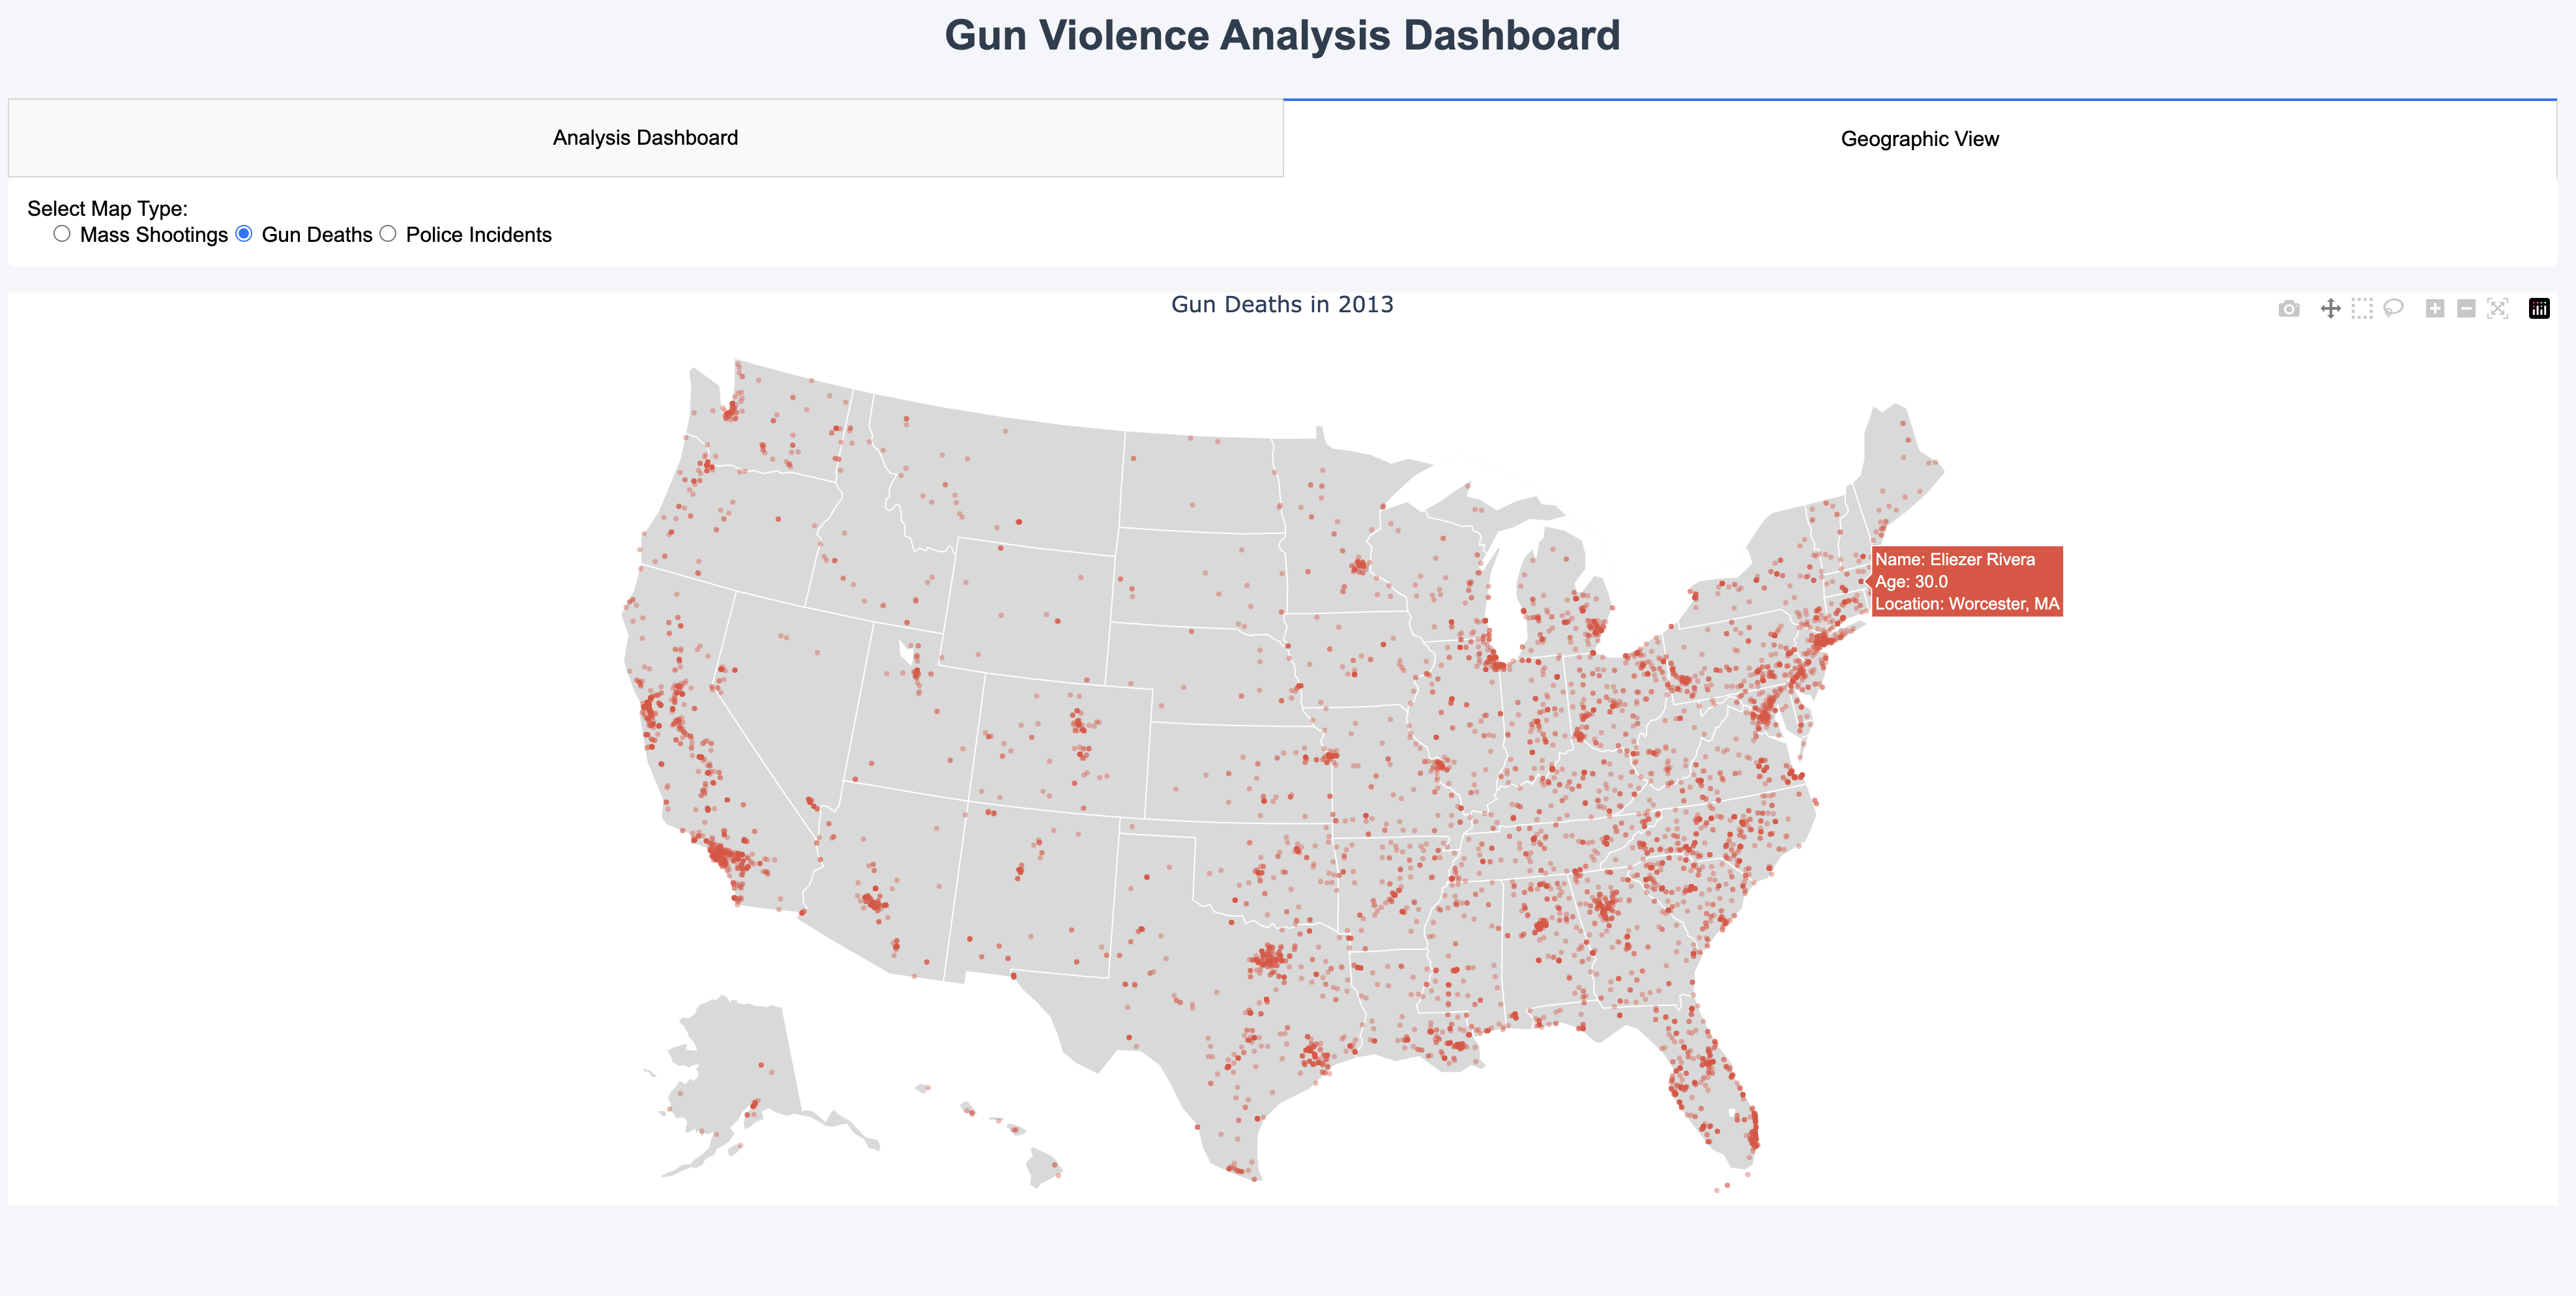
\includegraphics[width=0.9\textwidth]{GunDeaths.png}
    \caption{Geographic View of Gun Deaths. This map shows the distribution of gun-related deaths across the United States, with color intensity representing the frequency of incidents in each area.Users can hover over the orange dots to view the Name Age and Location of the victim.}
    \label{fig:gun_deaths}
\end{figure}

\begin{figure}[H]
    \centering
    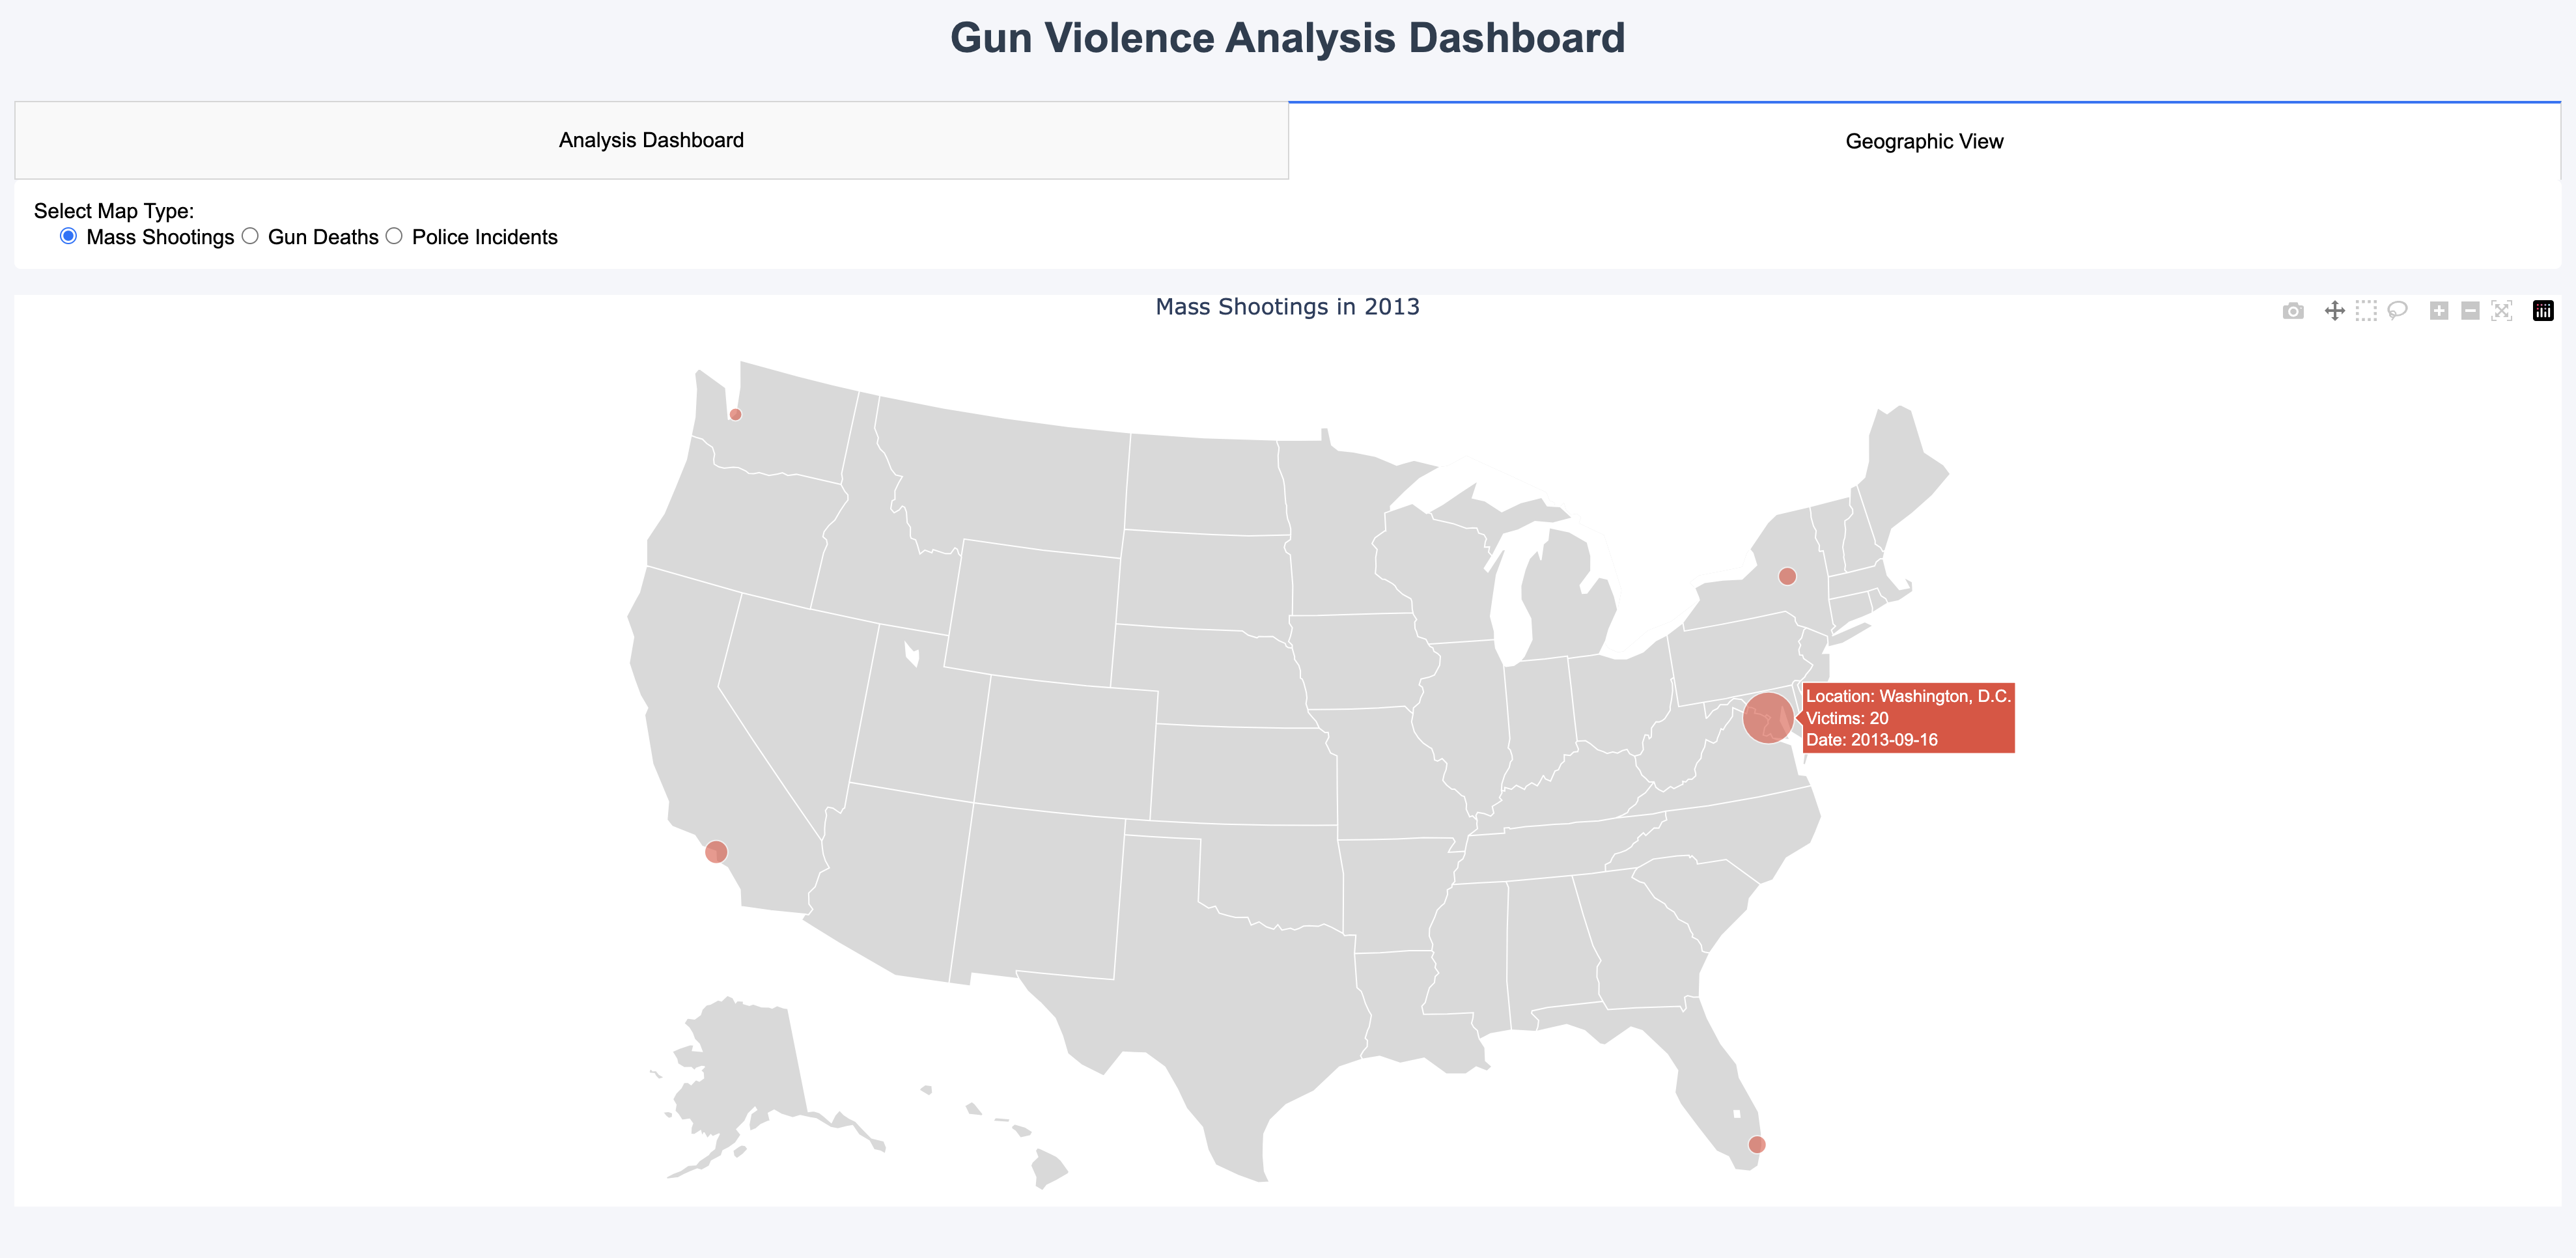
\includegraphics[width=0.9\textwidth]{MassShootingGeo.png}
    \caption{Geographic View of Mass Shootings. This map highlights regions affected by mass shooting incidents, allowing users to observe patterns in location and frequency.Users can hover over the orange region to view the Location, number of victims and the date of the dreaded incident.}
    \label{fig:mass_shootings}
\end{figure}

\begin{figure}[H]
    \centering
    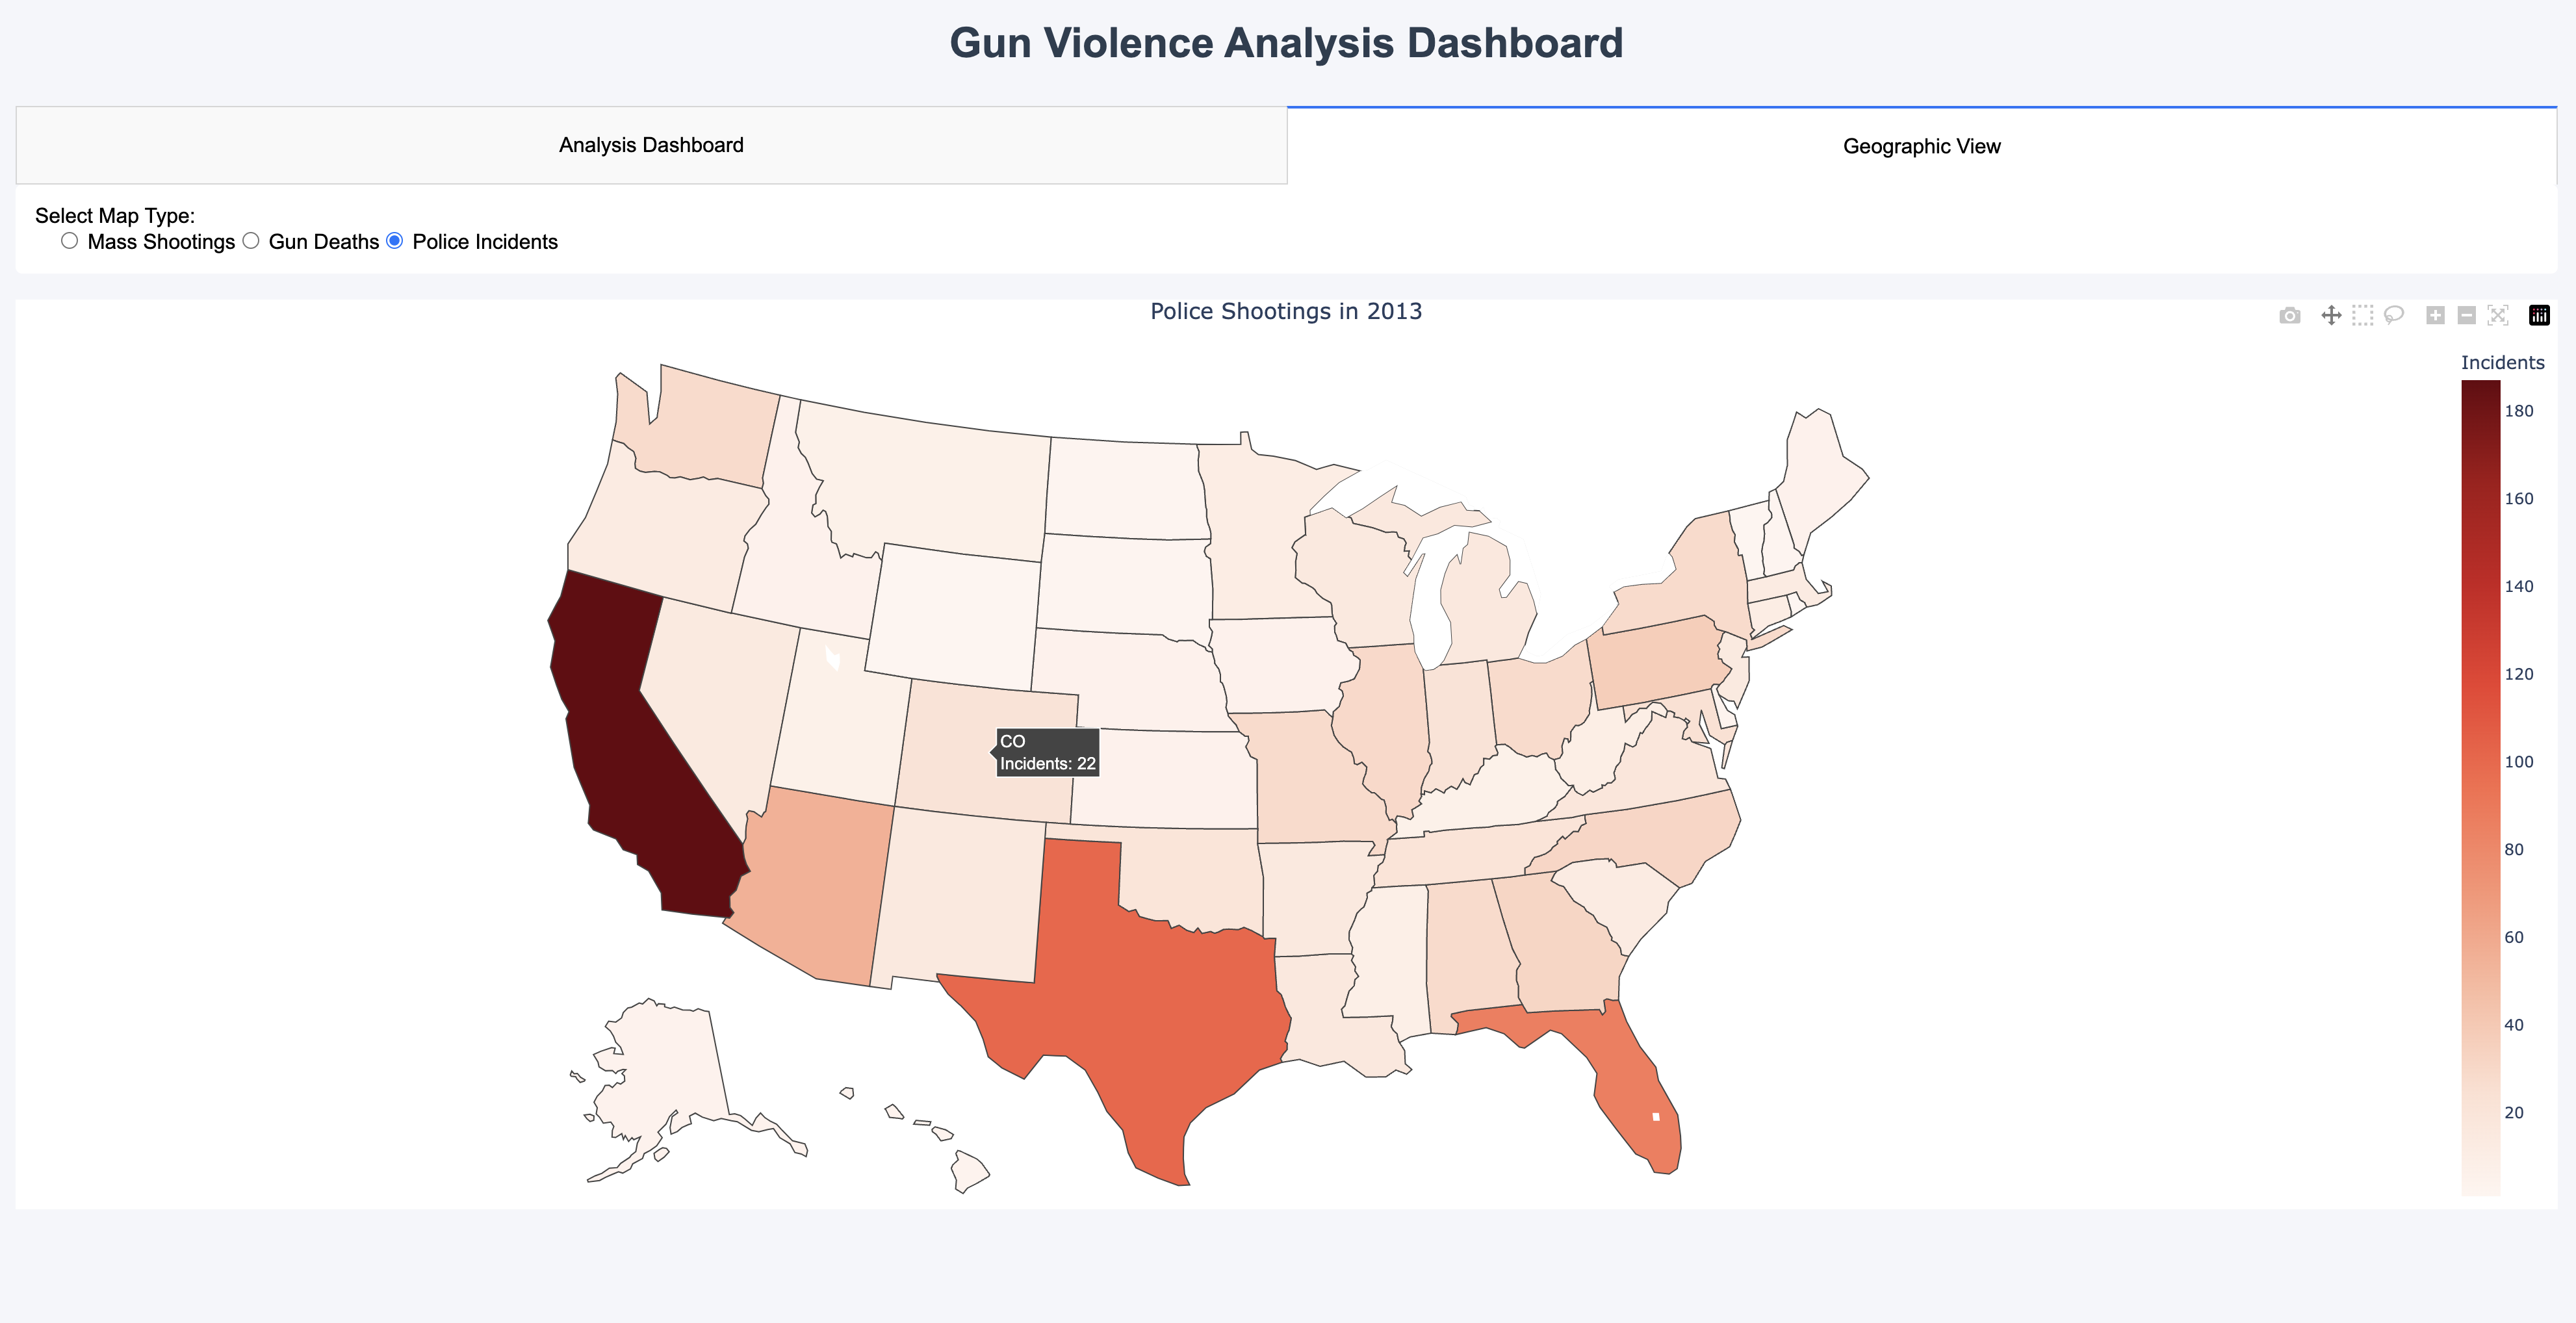
\includegraphics[width=0.9\textwidth]{policeIncedentGeo.png}
    \caption{Geographic View of Police Incidents. This map displays the distribution of police-related incidents, with darker colors indicating higher incident counts by region.Users can hover over each state to view detailed statistics, including the number of incidents reported in that area.}
    \label{fig:police_incidents}
\end{figure}

\begin{figure}[H]
    \centering
    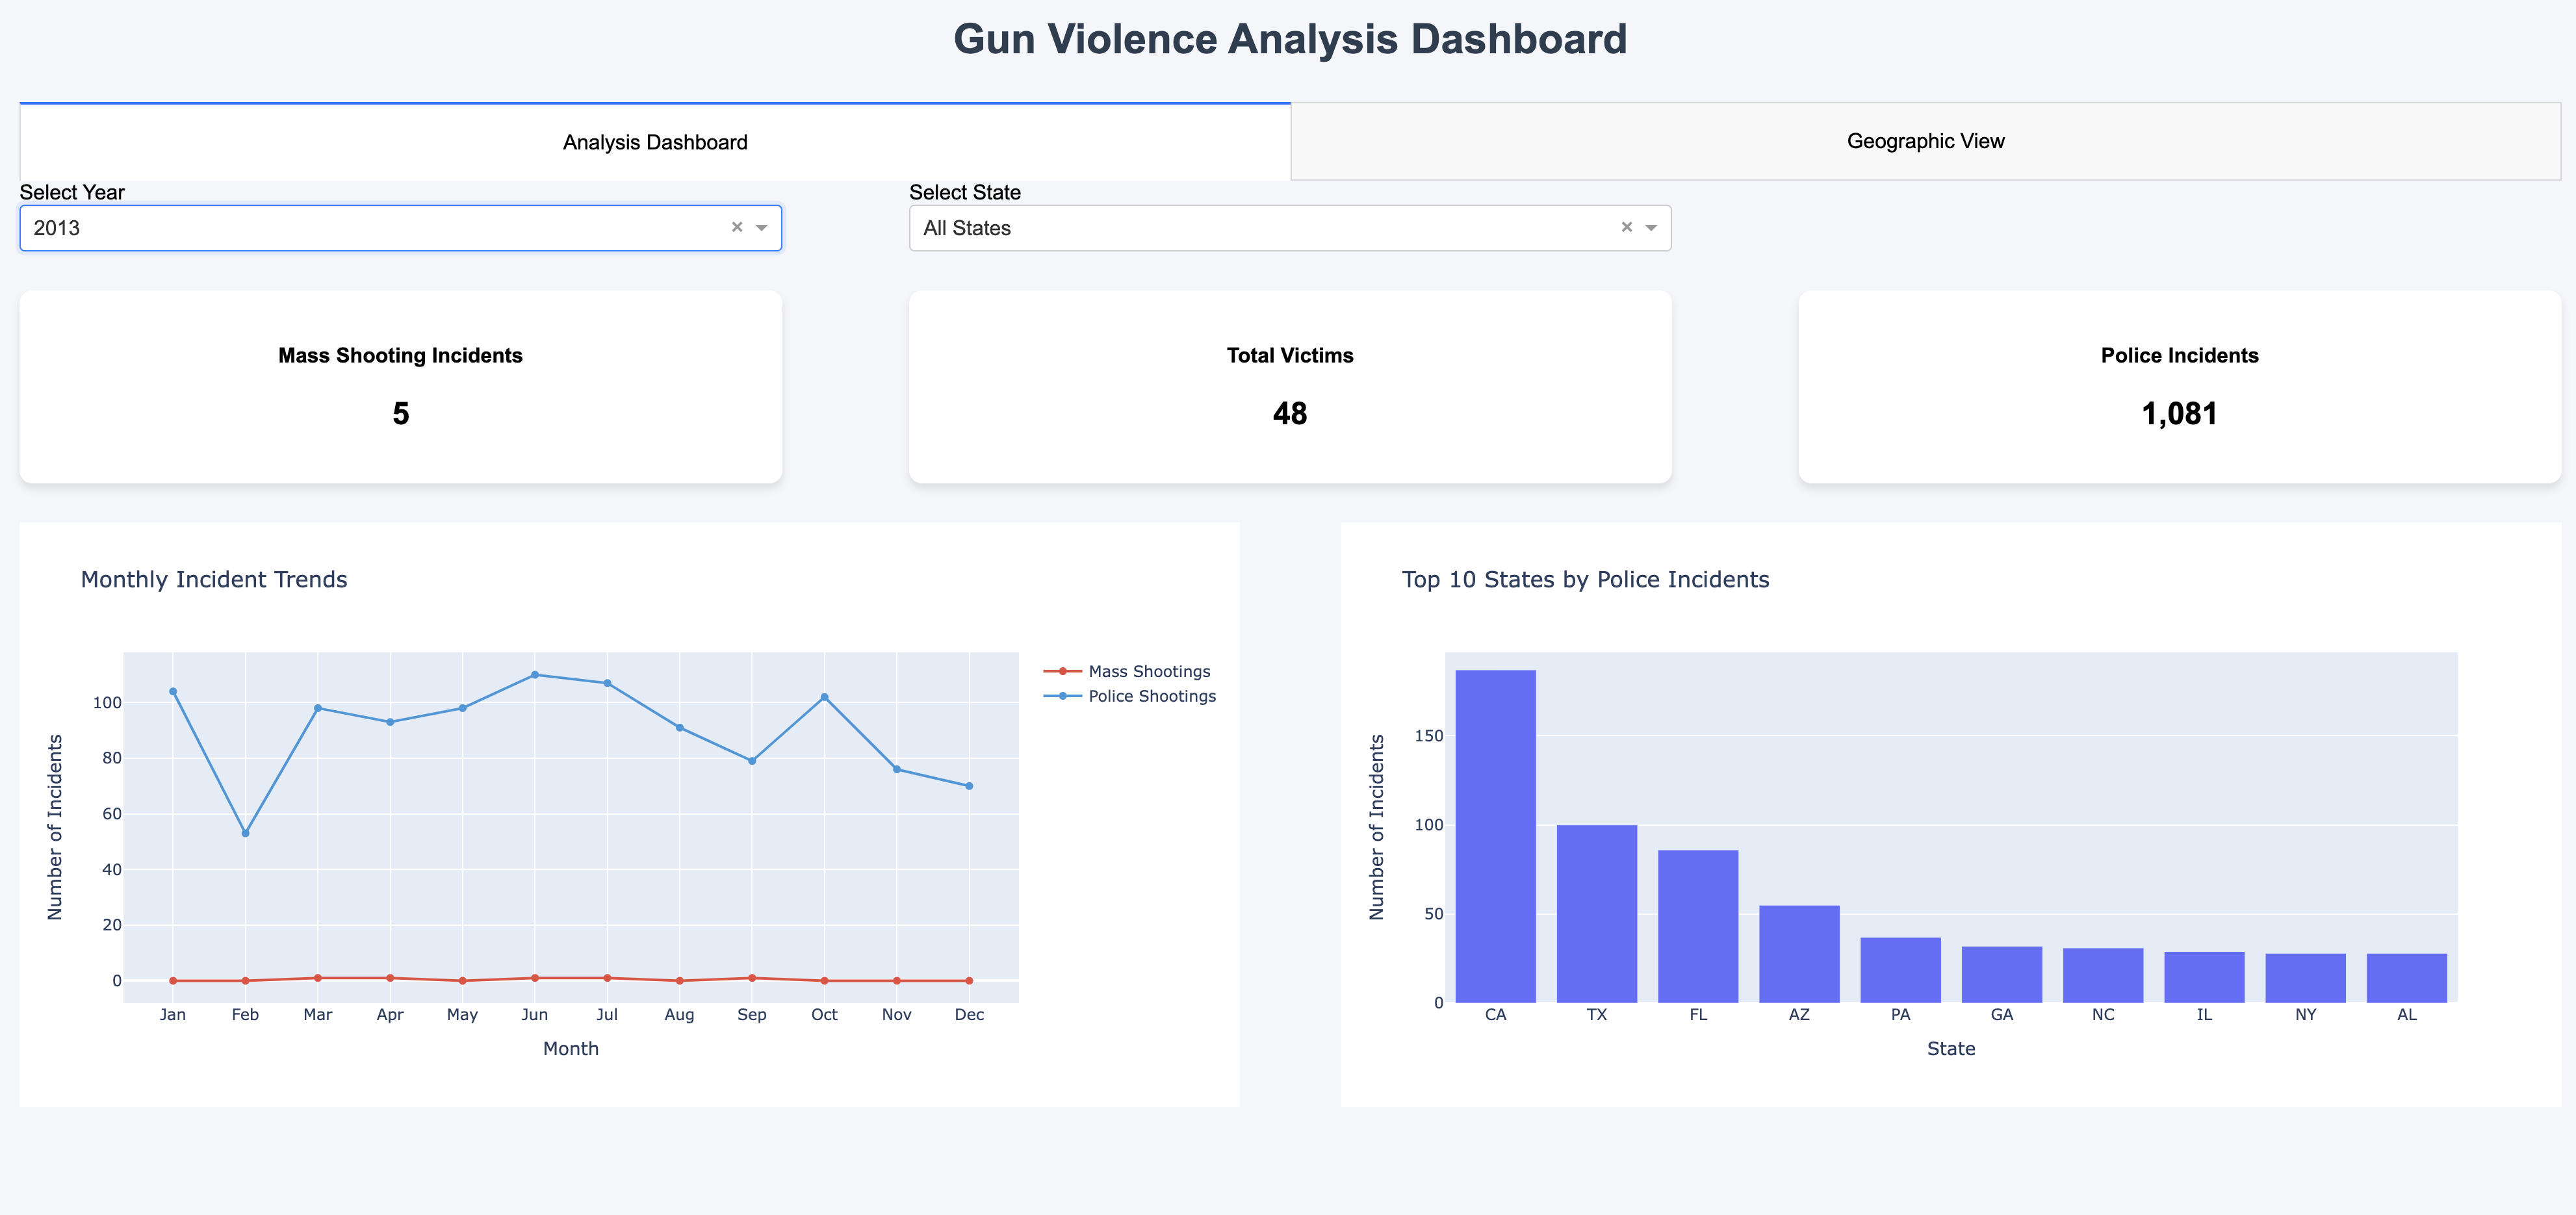
\includegraphics[width=0.9\textwidth]{AllStateView.png}
    \caption{Yearly Dashboard - All States. Provides a yearly overview across all states, including monthly trends and top states by incident count, to facilitate high-level analysis of gun violence patterns.}
    \label{fig:yearly_all_states}
\end{figure}

\begin{figure}[H]
    \centering
    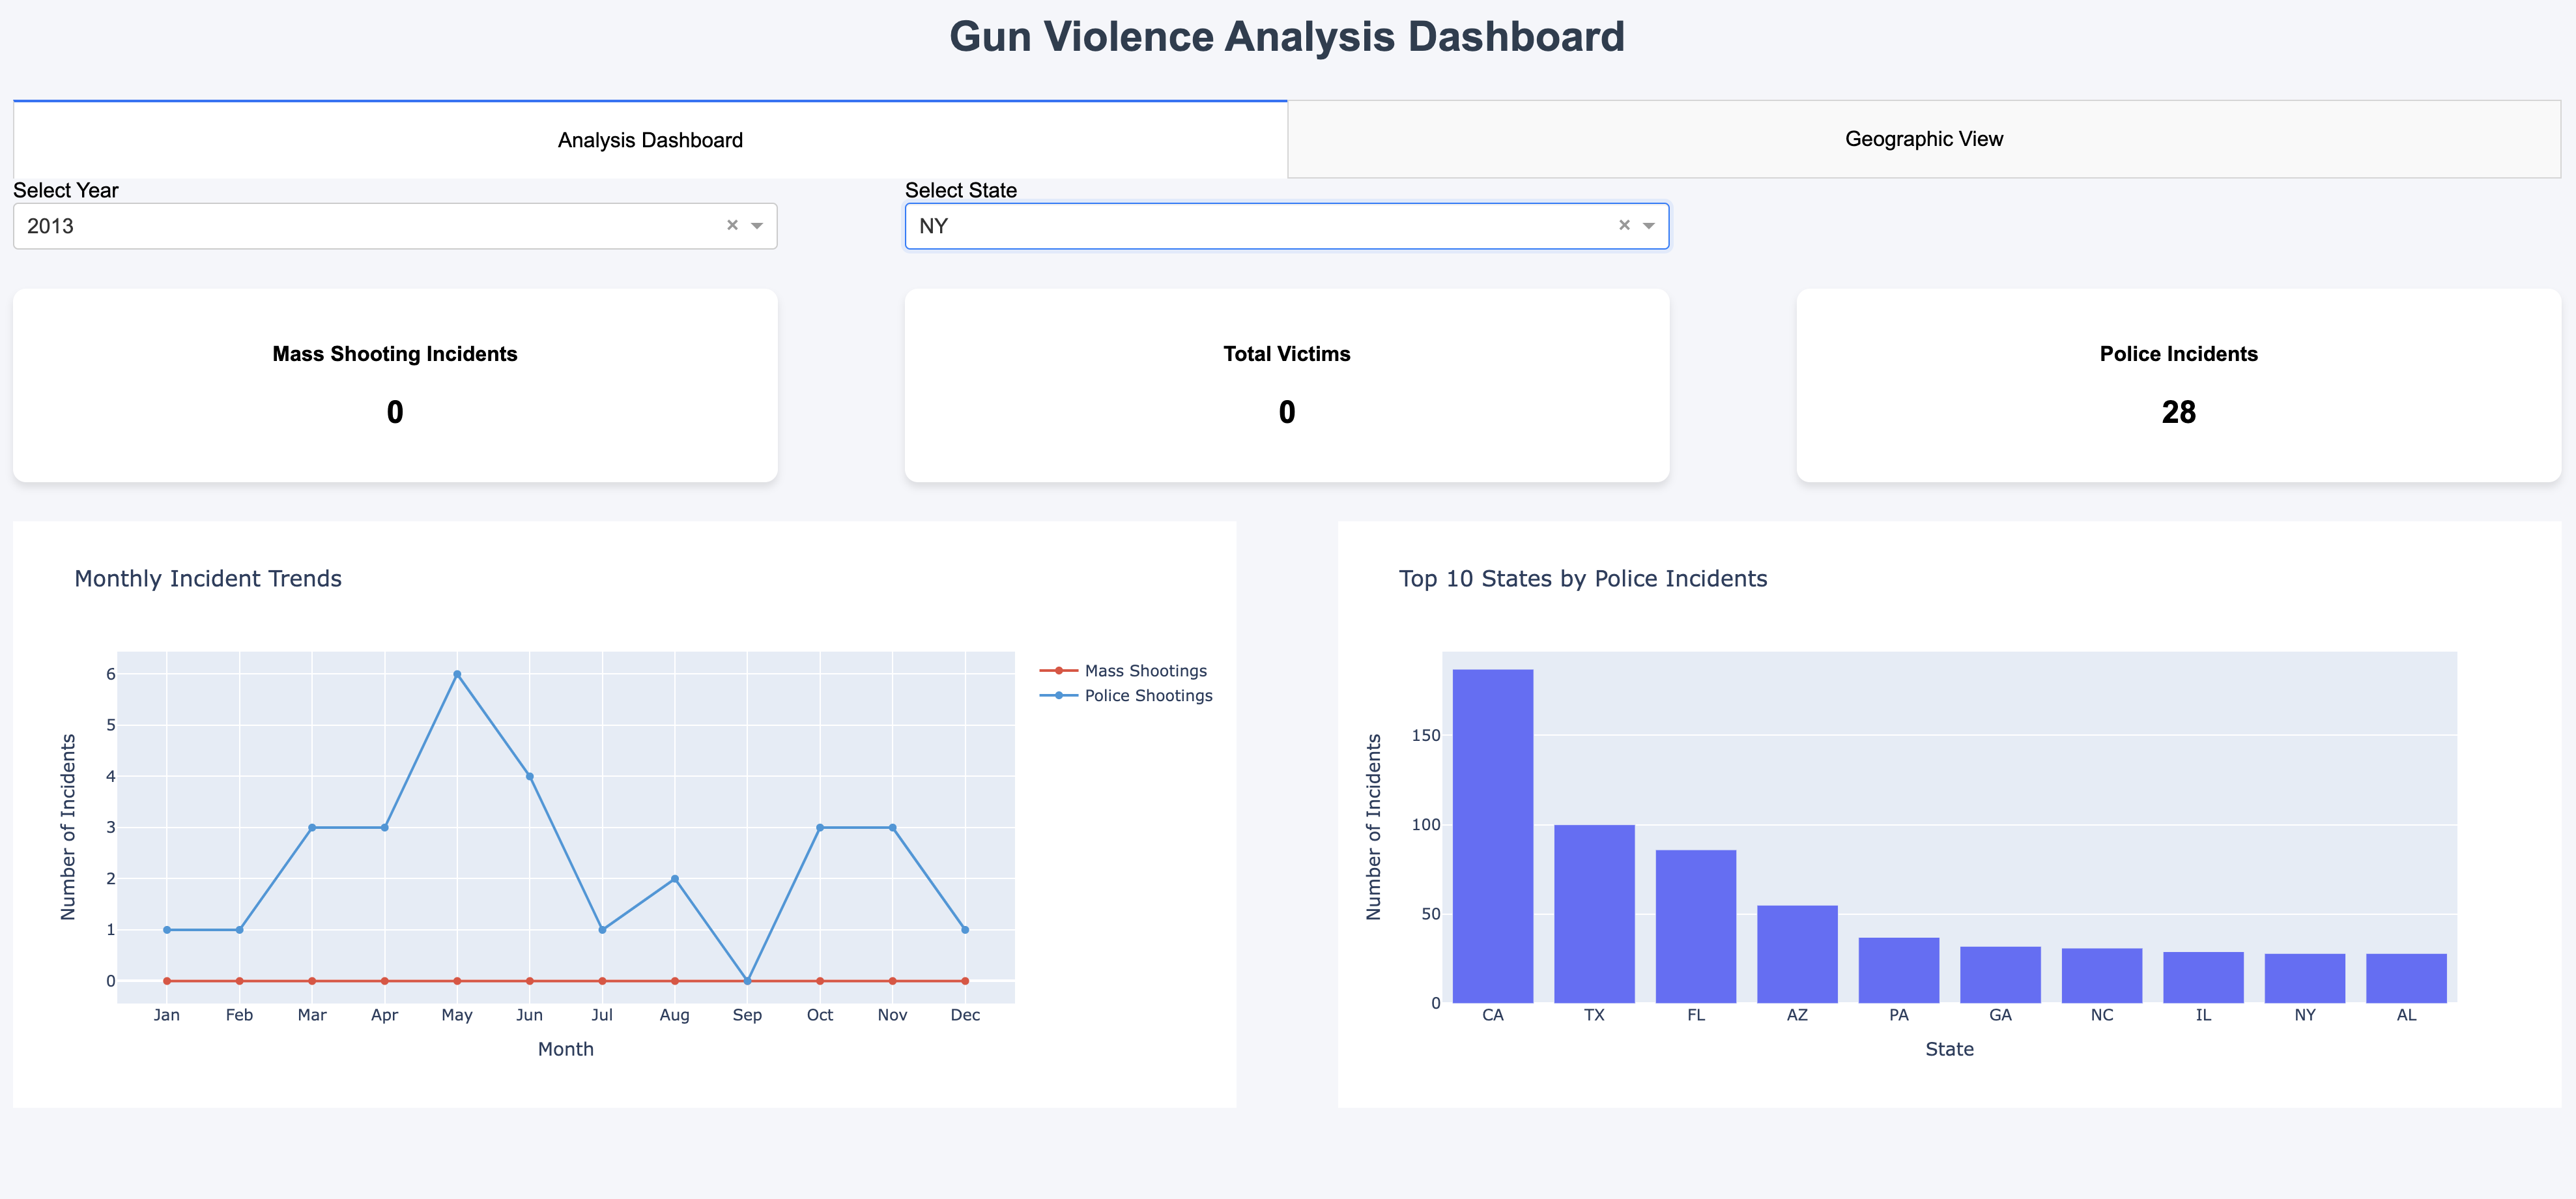
\includegraphics[width=0.9\textwidth]{NyStateView.png}
    \caption{Yearly Dashboard - Single State (NY). Allows focused analysis within a specific state, showing incident counts and monthly trends specific to the chosen region.}
    \label{fig:yearly_single_state}
\end{figure}

Each component was carefully designed to maximize clarity and usability:
\begin{itemize}
    \item \textbf{Geographic Views}: These views enable users to toggle between incident types, displaying distributions for gun deaths, mass shootings, and police-related incidents across the U.S. Color-coding highlights regions with higher incident frequencies.
    \item \textbf{Yearly Dashboard - All States}: This view provides an overview of incidents across all states for a selected year, showing monthly trends and top states by incident count.
    \item \textbf{Yearly Dashboard - Single State}: Focuses on a single state, allowing for in-depth analysis of monthly trends and incident counts within that state.
\end{itemize}

\section{Interaction Techniques}
The dashboard incorporates several interactive features:
\begin{itemize}
    \item \textbf{Dropdown Filters}: Users can select the year and state of interest, dynamically updating the visualizations to reflect the chosen parameters.
    \item \textbf{Map Toggle (Incident Type Selection)}: A radio button toggle lets users switch between mass shootings, gun deaths, and police incidents on the geographic map, enabling comparisons across incident types.
    \item \textbf{Tooltips}: On geographic views, hovering over a state reveals detailed incident counts, providing quick insights without additional clicks.
\end{itemize}

\section{Technical Implementation}
The dashboard was implemented using Python with Dash (version 2.14.2), leveraging its framework for building interactive web applications. Key aspects of the implementation include:

\begin{itemize}
    \item \textbf{Libraries and Tools}:
    \begin{itemize}
        \item Dash and Plotly for interactive visualizations and web interface
        \item Pandas for data preprocessing and manipulation
        \item NumPy for numerical computations
    \end{itemize}
    
    \item \textbf{Data Handling}: 
    The dataset is pre-processed with Pandas to clean, aggregate, and filter records. Data structures are optimized for quick retrieval and visualization, with implementation of caching mechanisms to improve performance.
    
    \item \textbf{Callbacks for Interactivity}: 
    Dash's callback functions manage real-time updates to graphs and maps based on user inputs (year, state, and incident type). Multiple callbacks coordinate the views across different visualizations.
    
    \item \textbf{Deployment}: 
    The completed dashboard is deployed on Render cloud platform, making it accessible as a web-based tool with configured error handling and logging.
\end{itemize}

The implementation focuses on maintaining a balance between performance and user experience, ensuring smooth interaction even with large datasets.

\section{Evaluation}
\subsection{Strengths}
\begin{itemize}
    \item \textbf{Intuitive Interface}: The layout and interactive components provide an accessible way for users to explore complex data.
    \item \textbf{Flexible Analysis}: The ability to filter by year, state, and incident type allows for tailored analyses based on user needs.
    \item \textbf{Comprehensive Views}: The dashboard combines geographic and analytical views, enabling users to examine both spatial and temporal trends.
\end{itemize}

\subsection{Weaknesses}
\begin{itemize}
    \item \textbf{Performance with Large Datasets}: Rendering may slow down with very large datasets, especially when filtering or toggling between views.
    \item \textbf{Limited Granularity}: Currently, data is visualized only at the state level; future versions could include county-level data for more granular insights.
\end{itemize}

\section{User Study and Feedback}
To evaluate the usability and effectiveness of the Gun Violence Analysis Dashboard, a user study was conducted with five participants, each of whom provided feedback through a Google Form. The participants were asked to rate the dashboard based on three criteria: overall usefulness, ease of navigation, and likelihood of recommending it to others.

\begin{figure}[H]
    \centering
    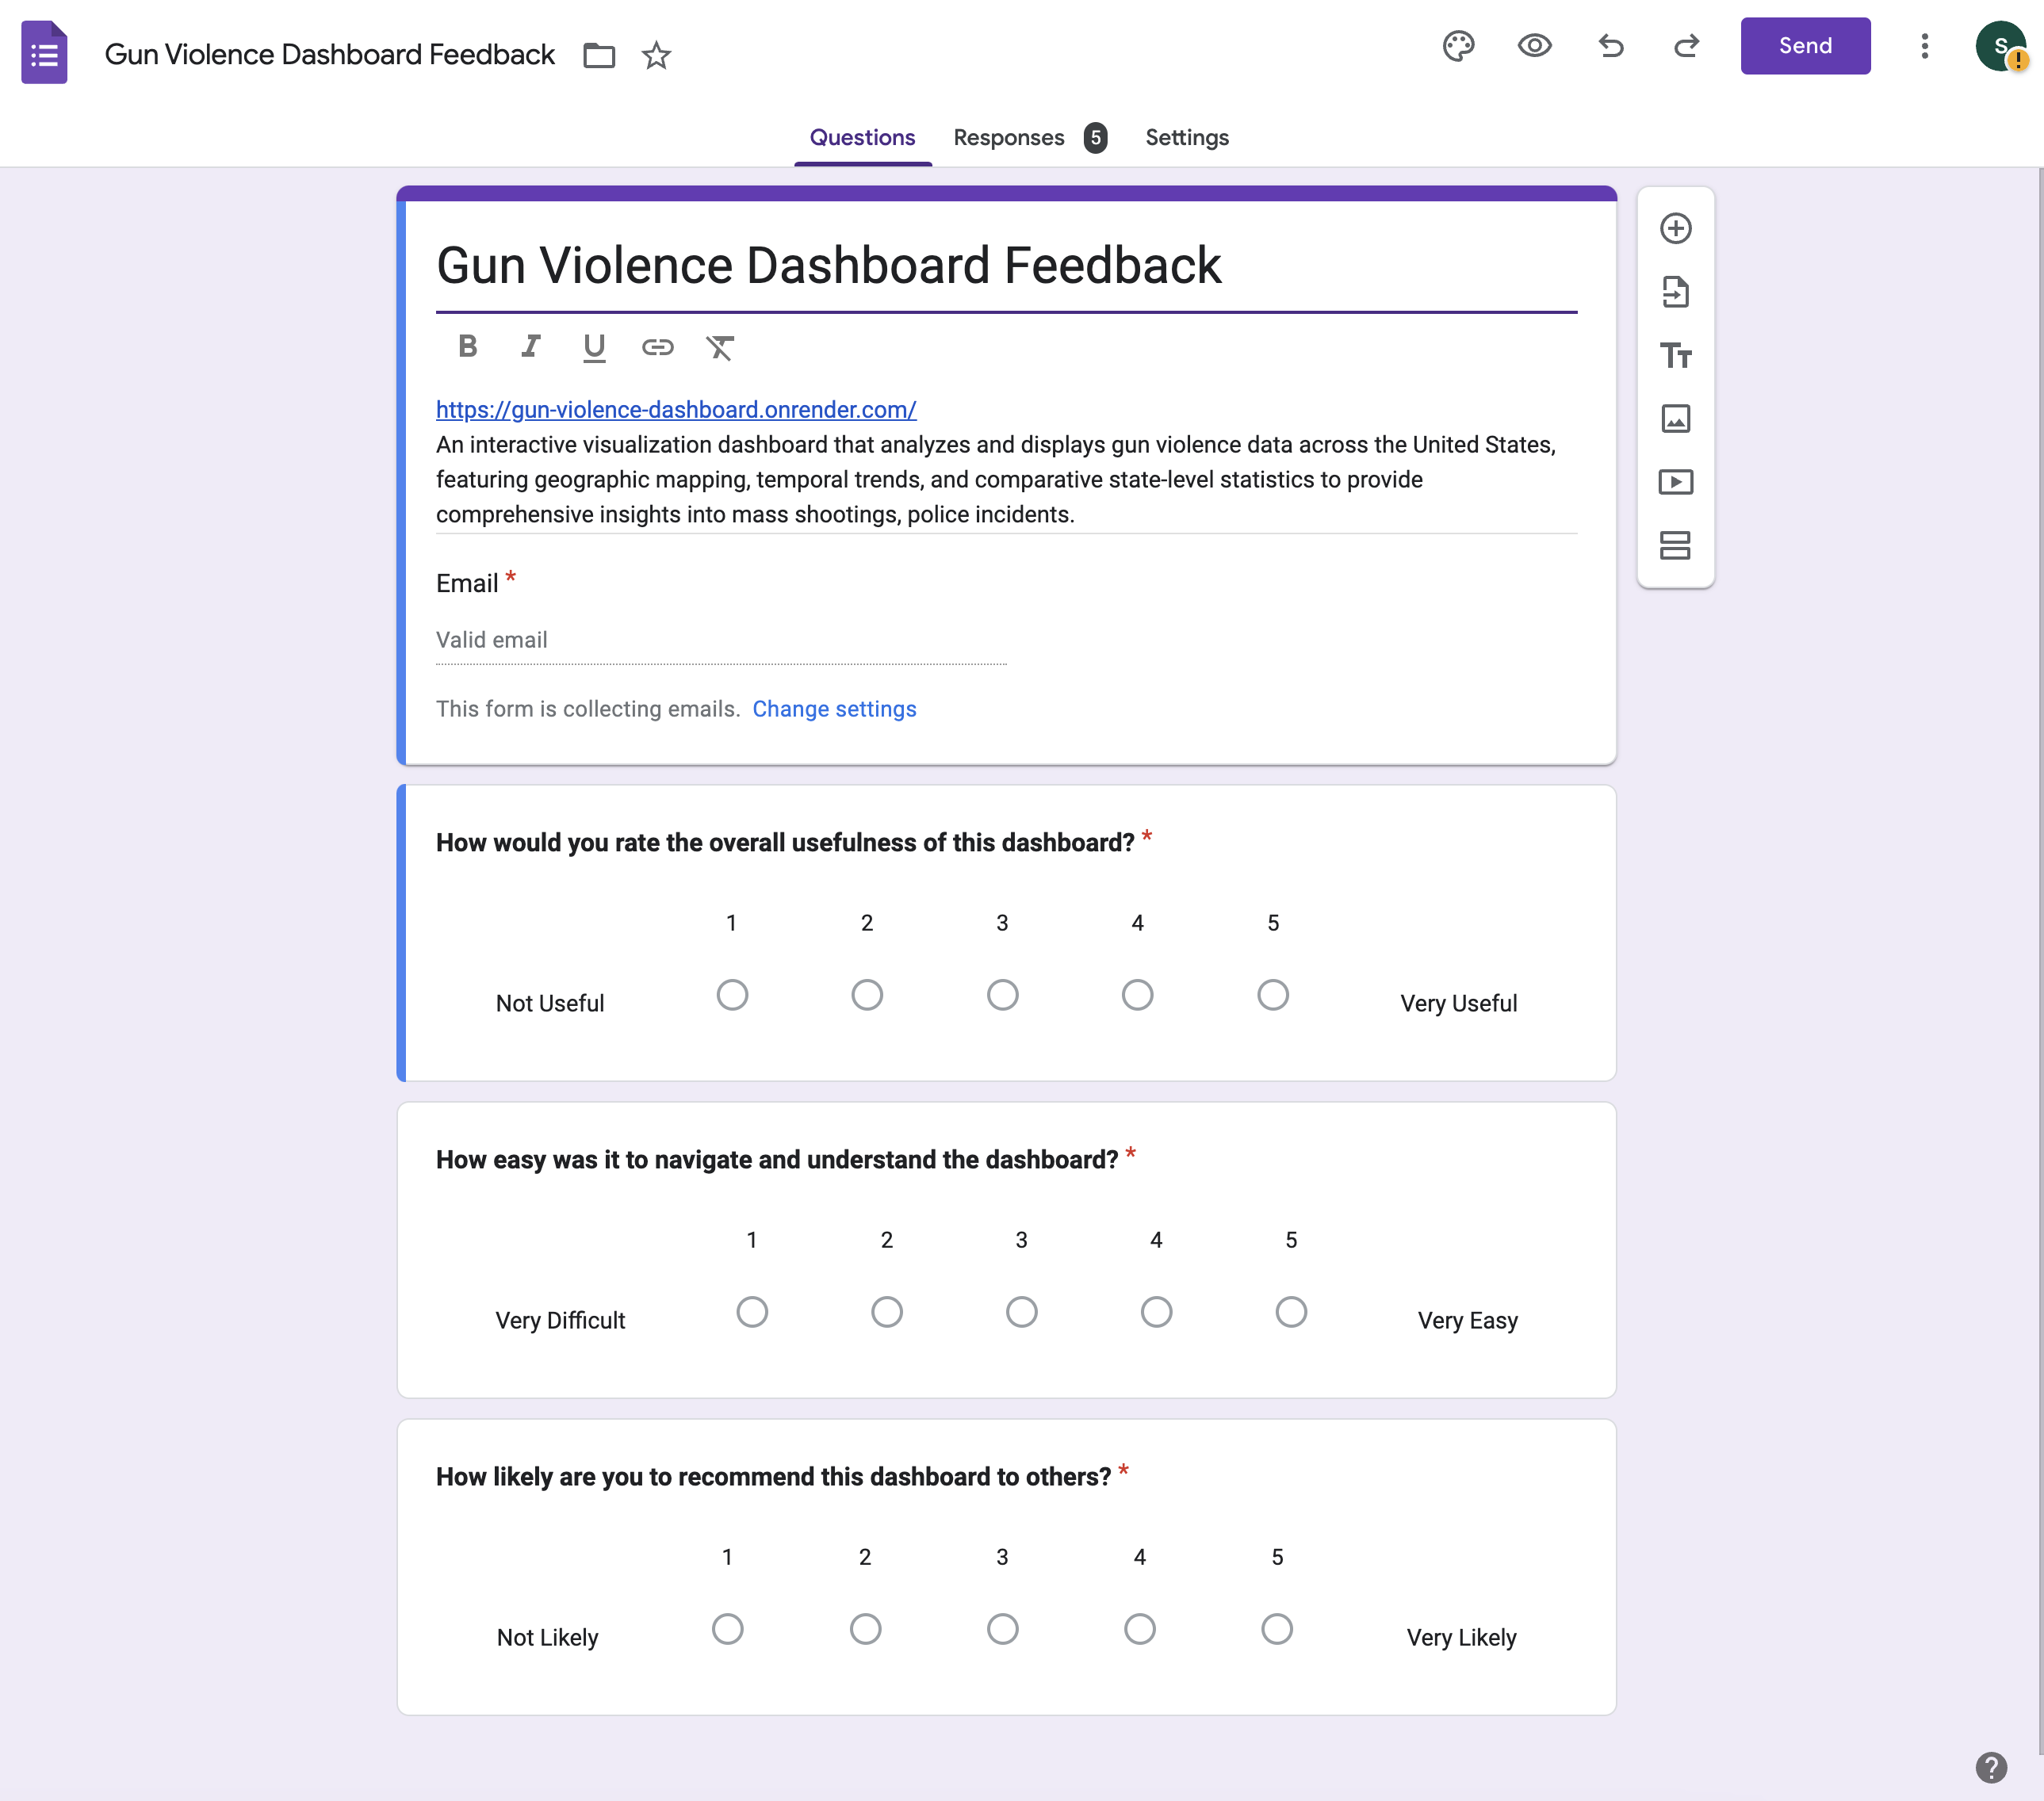
\includegraphics[width=0.9\textwidth]{GoogleForm.png}
    \caption{Google Form used to collect user feedback.}
    \label{fig:google_form}
\end{figure}

The collected responses indicate a positive reception of the dashboard:

\begin{itemize}
    \item \textbf{Overall Usefulness}: 80\% of respondents rated the dashboard as "Very Useful," while 20\% rated it slightly lower, indicating strong general approval of its functionality.
    \item \textbf{Ease of Navigation}: 60\% found the dashboard "Very Easy" to navigate, with the remaining 40\% rating it as moderately easy, suggesting that most users found the interface intuitive.
    \item \textbf{Recommendation Likelihood}: 80\% of participants stated they were highly likely to recommend the dashboard to others, showing confidence in its utility and appeal.
\end{itemize}

The feedback provided insights into areas of strength and suggestions for improvement:

\begin{itemize}
    \item \textbf{Positive Feedback}: Users appreciated the dashboard’s ability to switch between incident types and the interactive features that allowed detailed exploration of incident data by state and year.
    \item \textbf{Suggestions for Improvement}: Some participants recommended adding more granular data, such as county-level details, and enhancing the tooltips to provide additional context.
\end{itemize}

The responses, shown in Figures \ref{fig:google_form_response1} and \ref{fig:google_form_response2}, illustrate the distribution of ratings for each question.

\begin{figure}[H]
    \centering
    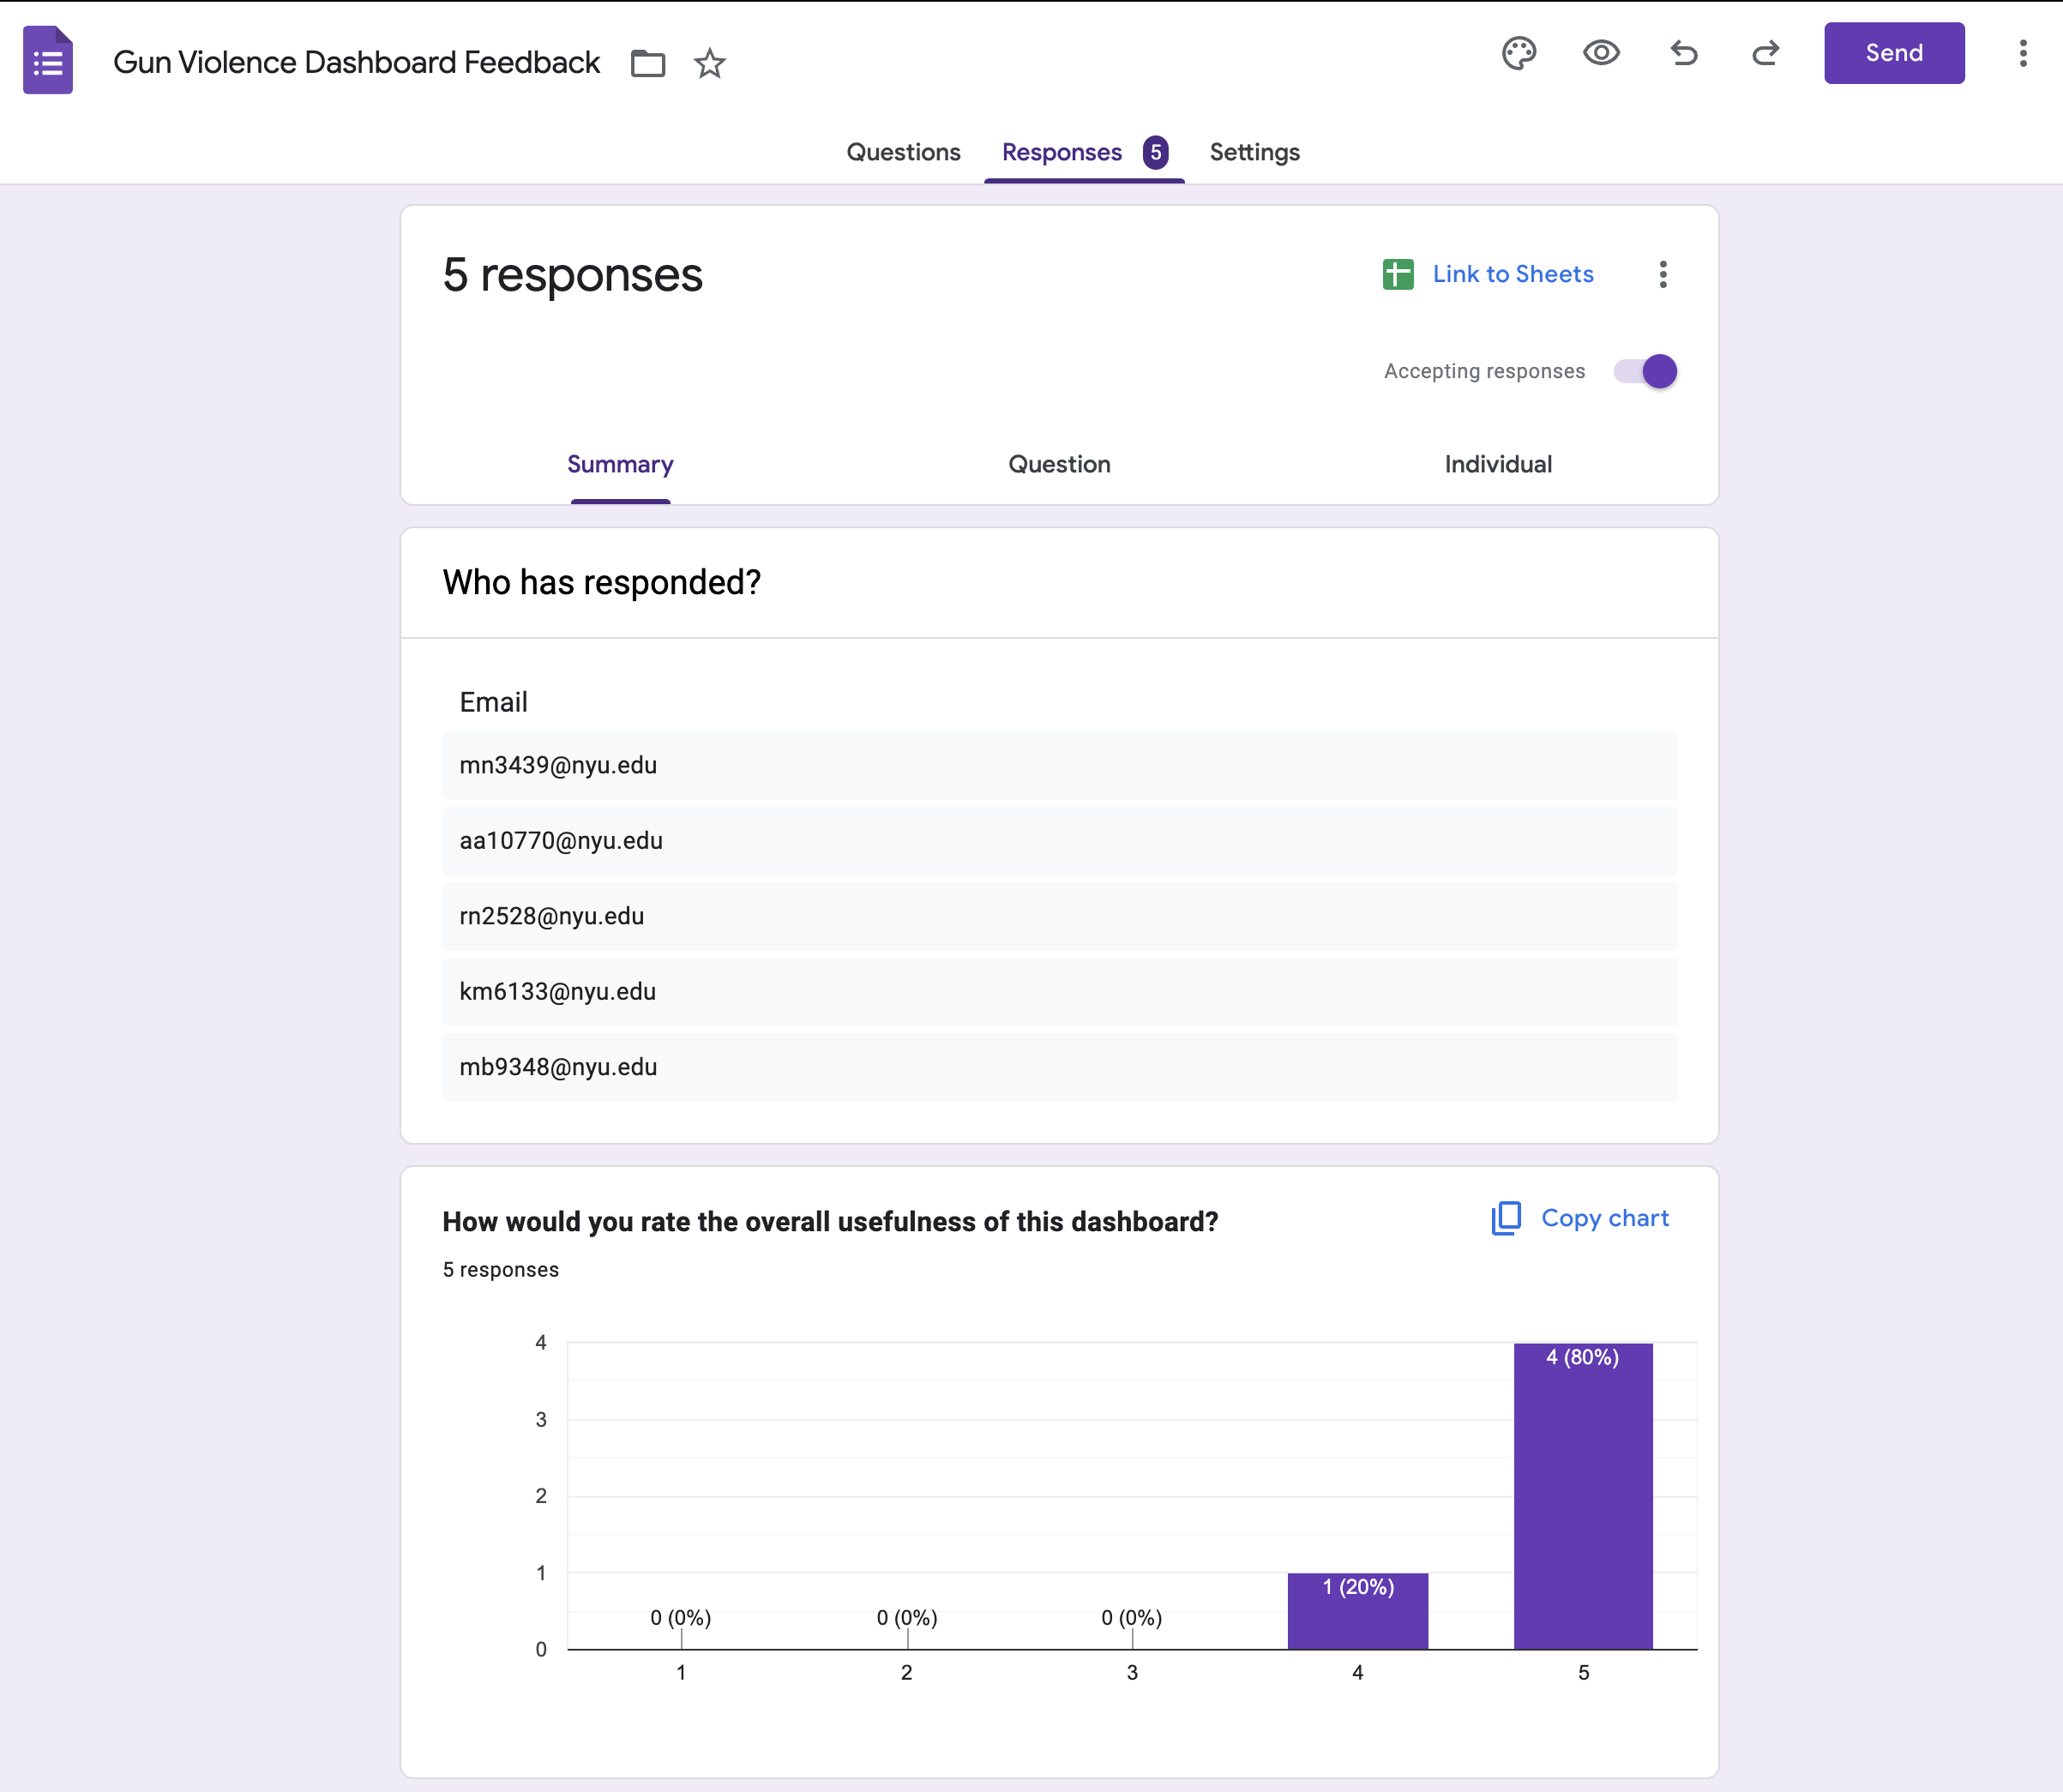
\includegraphics[width=0.9\textwidth]{GoogleFormResponse1.png}
    \caption{Responses to the question on overall usefulness of the dashboard.}
    \label{fig:google_form_response1}
\end{figure}

\begin{figure}[H]
    \centering
    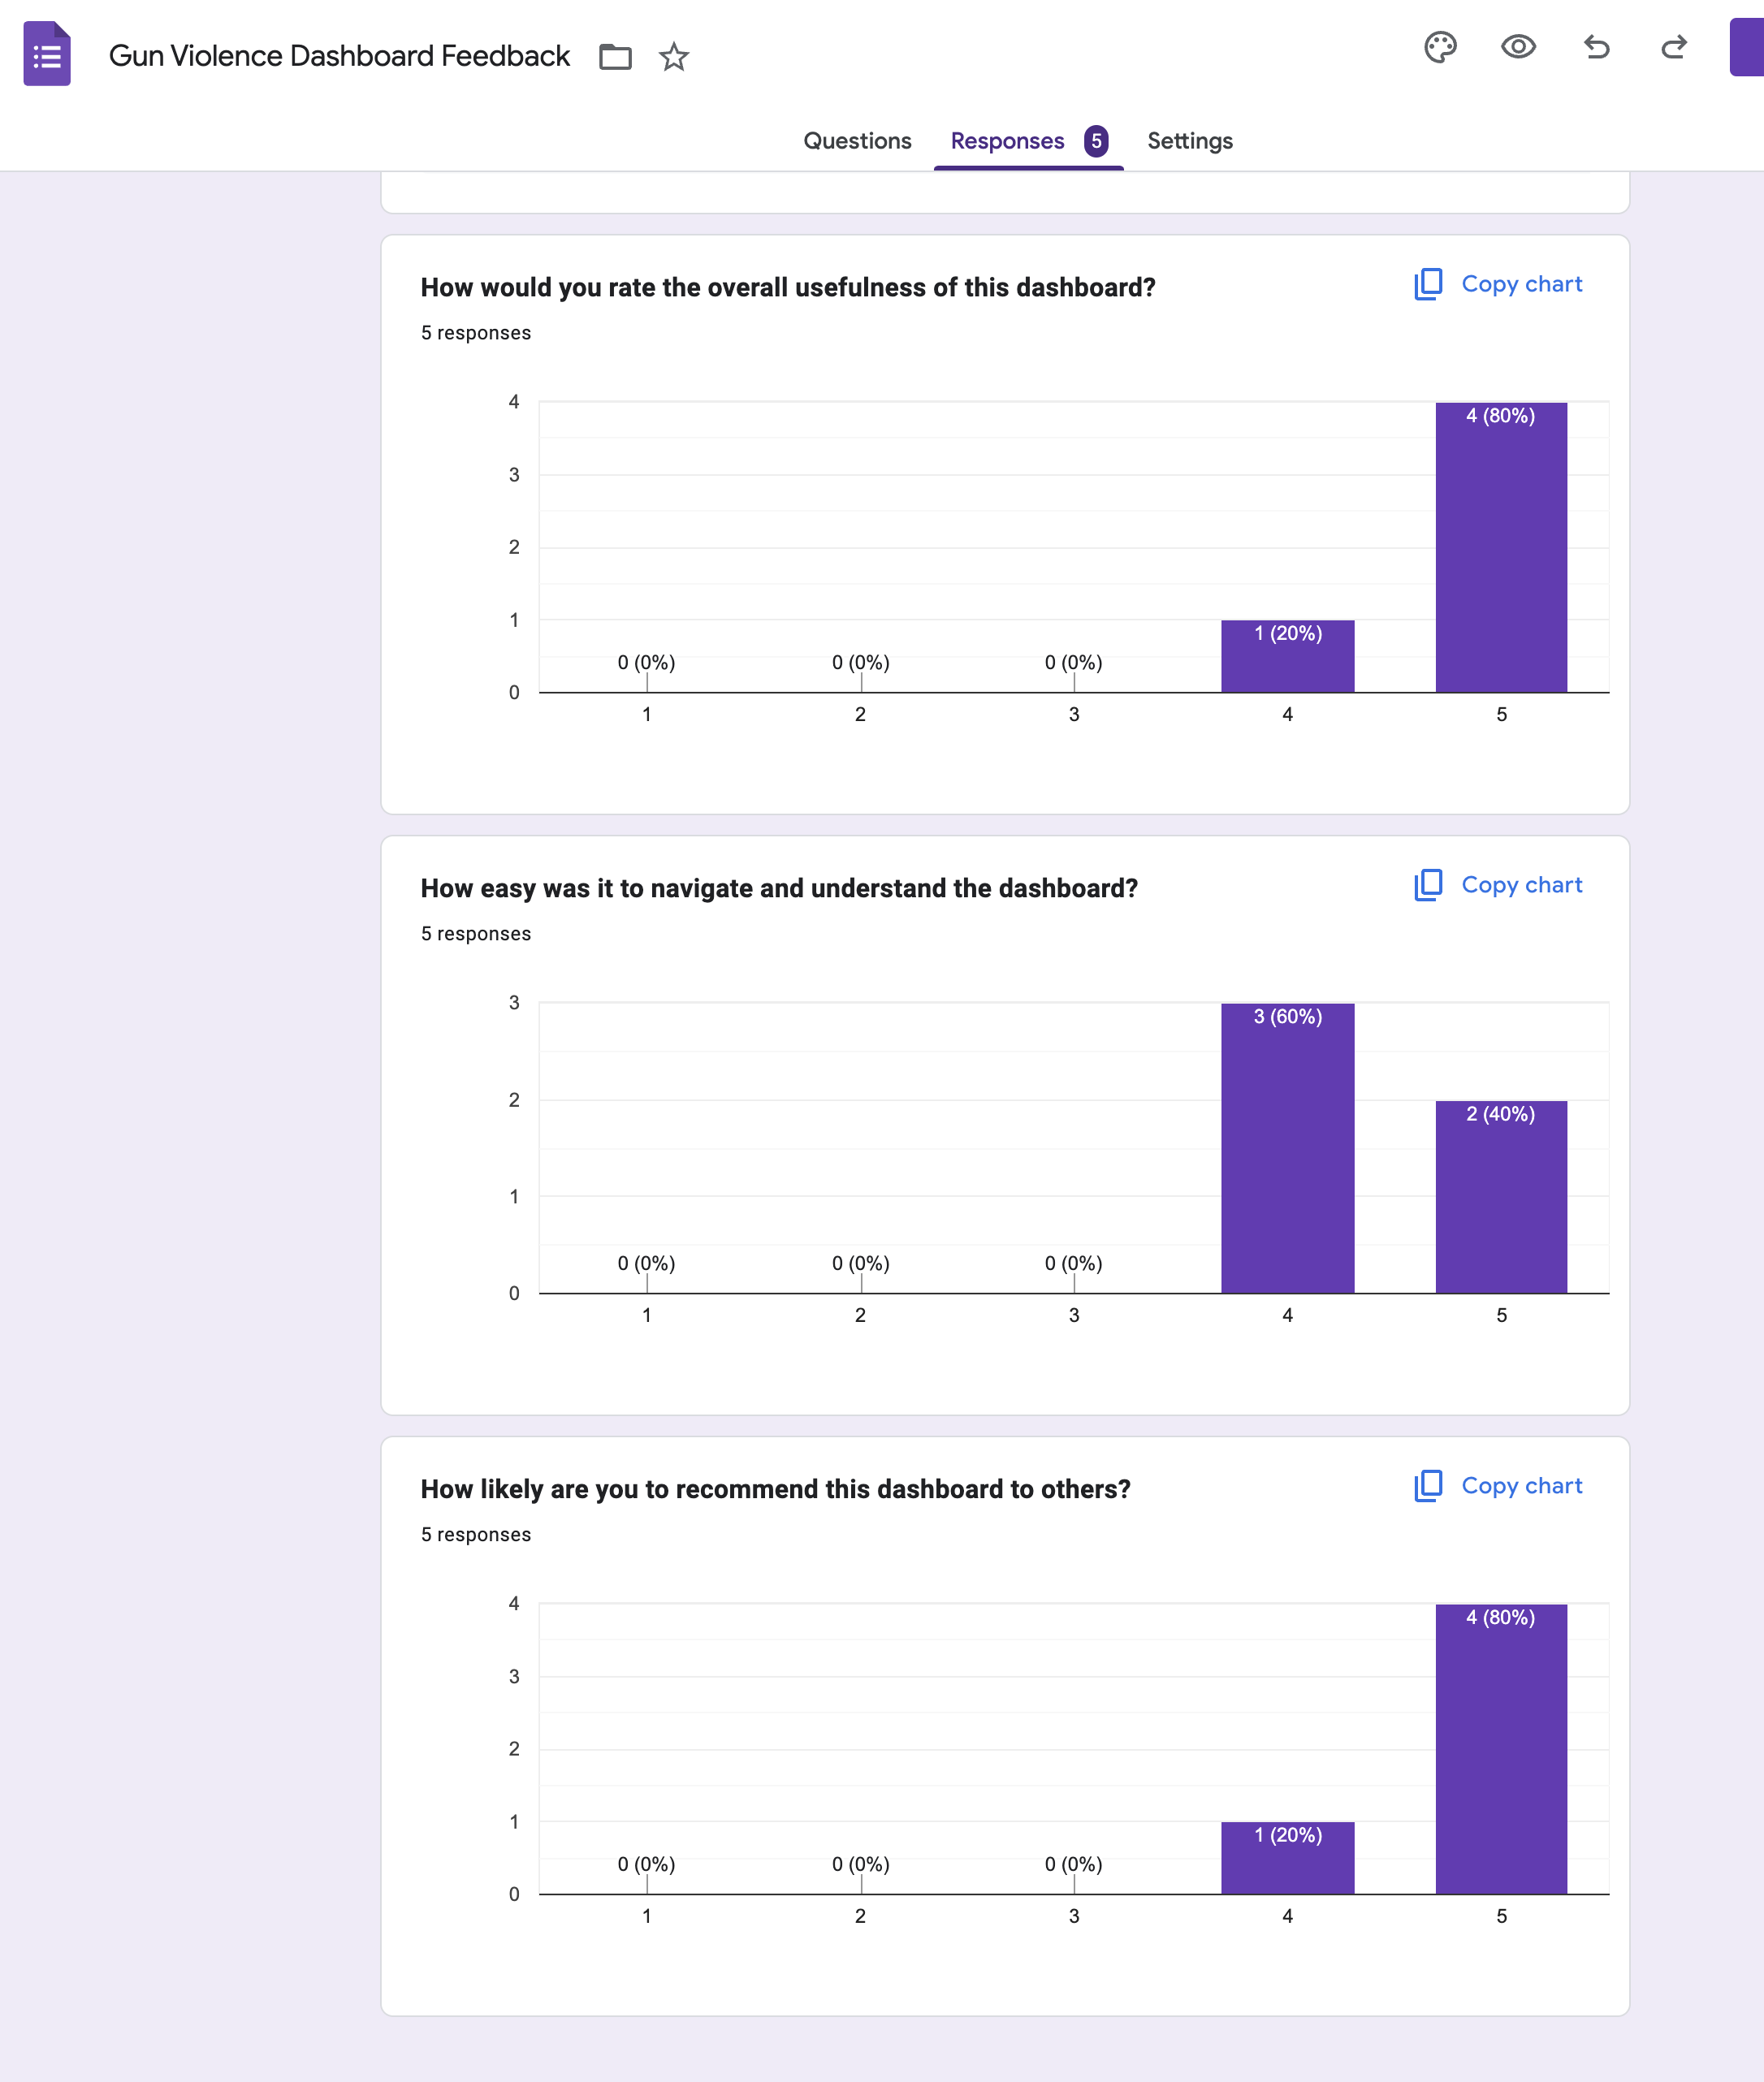
\includegraphics[width=0.9\textwidth]{GoogleFormResponse2.png}
    \caption{Responses to the questions on ease of navigation and likelihood of recommendation.}
    \label{fig:google_form_response2}
\end{figure}

Overall, the user study provided valuable insights that validated the dashboard’s effectiveness while highlighting potential enhancements for future versions. The high scores in user satisfaction metrics reflect the dashboard’s success in meeting user needs and expectations.

\section{Conclusion}
The Gun Violence Analysis Dashboard effectively meets its objective of providing a comprehensive tool for visualizing and analyzing gun violence data in the United States. By incorporating interactive elements such as filtering, tooltips, and multiple view options, the dashboard allows users to explore complex data with ease and flexibility. 

The dashboard’s design choices, which include both geographic and analytical views, make it versatile for users interested in spatial and temporal patterns of gun violence. The positive feedback from the user study confirms the dashboard’s usefulness and ease of navigation, while also pointing out areas for future improvement, such as adding more granular data.

Overall, this project demonstrates the potential of interactive visualizations in presenting large-scale data in an accessible format, supporting informed decision-making and further research on critical issues like gun violence.

\end{document}
